\documentclass{ICASP13Paper}

% Add an "addauthor" line for each author with the following syntax:
% \addauthor{Name Initials Surname}{Title and affiliation}
\addauthor{Jane M. Smith}{Professor, Dept. of Civil Engineering, Univ. of 
Reliability, City, Country}
\addauthor{John M. Smith}{Graduate Student, Dept. of Civil Engineering, Univ. 
of Reliability, City, Country}
\addauthor{Jonny M. Smith}{Research Engineer, Reliability Consultants Inc., 
City, Country}

% The title of the abstract
\title{Probabilities in Practice}

% The bibtex reference file where the references should be found
\referencefile{bib}

% Short abstract of the paper
\shortabstract{The abstract is written last, when the paper is complete. It 
contains a summary of the paper, usually starting with a few words about the 
objectives. Thereafter follow usually statements about the importance of the 
work and the methodology that is employed. The key results are then summarized 
followed by an overview of the conclusions that were drawn from the study.}

\begin{document}
The ICASP conferences are held every four years and seek to gather researchers 
and practitioners to present and discuss the state-of-the-art in probability 
and statistics applied to civil engineering problems. Professors and leading 
practitioners are particularly encouraged to make presentations because their 
experience will allow them to include comments about where they think the 
discipline should go in the future.
\par
Authors who were invited to submit a full paper are asked to follow the 
guidelines posted at the conference website. That includes using this document 
as a template. This document is created in Word using “styles,” which define 
the format of each paragraph. Notice for example that the paragraph above has 
the style Firstparagraph, implying that there is no indentation of the first 
line.
\par
That style should be applied to every paragraph that follows immediately after 
a heading. It is also an appropriate style immediately after equations, when 
the text is a natural continuation of the equation. In contrast, the Normal 
style assigned to this paragraph features an indentation of the first line.
\par 
In regards to styles, it is also noted that the title of the paper is assigned 
the Title style. The capitalization of the first letters must be done manually. 
After the title follows the Authorname and the Authoraffiliation styles. All 
styles in this document employ the Times New Roman font type, but the font 
sizes differ. The title is 18pt, the author names are 14pt, the author 
affiliations are 12pt, the Normal text is 12pt, the captions and references are 
11pt, and the header is 10pt.
\par
The space allocated to the author list is elastic; the more authors the more 
space it will take. There is a concealed Section Break after the author list 
that provides this elasticity. Section breaks are part of the hidden codes, 
i.e., nonprinting characters in Word. If you encounter strange problems with 
this document then one reason might be that you are unaware of hidden codes. In 
this document the most important nonprinting character is the Section Break in 
the empty paragraph immediately after the last author affiliation.
\begin{figure}[h!]
  \centering
  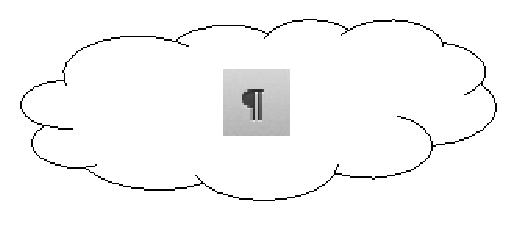
\includegraphics[scale=0.6]{Cloud}
  \caption{Nonprinting characters in Word (notice the line break below this 
  caption, to provide some air). }
  \label{fig:label}
\end{figure}  
\par
In addition to the abovementioned elasticity, the section break is required to 
facilitate the two-column format and must not be removed. To view it, press the 
appropriate toolbar button in Word, shown in Figure~\ref{fig:label}. 
\par
Notice that the above reference to a figure is inserted by using the 
cross-reference feature in Word. Although slightly more cumbersome, this can 
also be done also for equations such as
\begin{equation} \label{eq:label}
  p_f = \varPhi(-\beta)
\end{equation}
where the Equation style is used and the equation number is a caption, i.e., it 
turns grey if you drag the cursor over it. That means that it can be referenced 
elsewhere, and doing so requires three magic steps. First, temporarily insert a 
line-break immediately before the opening parenthesis of the equation number. 
Second, write Eq. where you want to reference the equation and insert a 
Cross-reference from the Insert menu, using the “Entire caption” option. The 
result is Eq.~(\ref{eq:label}). Third, remove the line-break that you inserted 
in the first step. Also note that this paragraph, immediately following an 
equation, has the Firstparagraph style to avoid indentation of the sentence 
that forms a continuation of the equation.
\begin{table}[h!]
  \caption{Parameter values.}
  \label{tab:label}
  \centering
    \begin{tabular}{|c|c|c|}
      \hline
      a & b & c \\
      \hline
      1.0 & 2.0 & 3.0 \\
      \hline
    \end{tabular}
\end{table}
\par
An example of a table is also included in this template and the reference to it 
is Table~\ref{tab:label}. Again notice that this is a cross-reference that is 
automatically updated. Borderlines in the table may be removed if it improves 
readability. Finally, if citations are needed, then please use the ASCE 
citation format \cite{Kiureghian2009}, making sure to cite all references that 
are included in the reference list.

\section{GOOD HABITS OF TECHNICAL WRITING}
A few ideas are provided in the following on how to create strong academic 
papers. These are not strict rules but perhaps some of them will be useful:
\begin{compactitem}
  \item Understand that a pedagogical presentation is as important as the 
  content; focus aggressively on clarity: First write, then rewrite and revise, 
  then put the text aside for a while before reviewing, rewriting, and revising 
  again.
  \item While focusing on a clear and inspirational presentation, never 
  compromise on technical quality and academic integrity.
  \item To improve your writing, study and imitate the style and phrasing of 
  publications that you find particularly clear and inspiring.
  \item Define who your readers are and continually imagine them reading what 
  you write.
  \item Always start writing a paper by spending significant time setting up a 
  bullet-itemized outline; a guideline is provided in the section below.
  \item Let each paragraph have one topic and provide meaningful links between 
  paragraphs to assist the flow of the text. Write grammatically active and 
  complete sentences in accordance with the rules that are described later in 
  this document.
  \item Continuously search for more formal words to replace informal ones; 
  this improves the style, clarity, and suitability of an academic paper
  \item Keep the sentences short and concise; mercilessly place each word on a 
  imaginary scale to test if it really justifies its presence.
  \item Avoid abbreviations unless they significantly improve the readability 
  and brevity of the subsequent text; if an abbreviation is necessary then 
  define it only once, where it first appears.
  \item Always describe and discuss the content of tables and figures in the 
  text, but do not duplicate data from those elements in the text.
  \item Avoid the use of boldface, italics, underline, parenthesis and other 
  importance labels in the text; state everything with words
\end{compactitem}

\section{PROPER INTRODUCTIONS}
Although a section named Introduction is not mandatory, the importance of the 
introductory part of a paper cannot be overemphasized. Although it does not 
contain the substance of the paper it sets the stage and establishes the tone 
of the paper. A poor introduction usually identifies a poor paper. A proper 
introduction may result from following these steps:
\begin{compactenum}
  \item Start with a thoughtful first sentence that concisely summarizes the 
  objective and why it is important; above all, inspire the reader to read on
  \item State the long-term goals and visions of the work
  \item State the short-term objectives that are specifically addressed to 
  achieve the long-term goals
  \item State the scope of the work to identify the problems that are, or are 
  not, considered
  \item Identify who has done what in the past. Sometimes, this review requires 
  a separate section. However, care should be exercised to avoid an 
  unnecessarily lengthy literature review. A concise and well-informed exposure 
  of the background fits in the introductory section.
  \item Depending on the complexity of the paper, provide an overview of the 
  sections. This type of overview is more common in books, reports, and theses 
  than in conference and journal papers.
  \item Identify the novelties of the paper to let the peer reviewer understand 
  that there is something new in this paper, and to let the general reader know 
  which highlights to look out for
\end{compactenum}

\section{THE MEAT OF THE PAPER}
Between the Introduction and the Conclusions there exist no mandatory section 
organization. The outline depends strongly on the work that is carried out. The 
following two sections provide one suggested organization of the content.

\subsection{Methodology}

\subsubsection{Build-up}
Bring the reader up to speed on the existing methodology; be brief

\subsubsection{Developments}
Explain the new use, merger, or extension of the methodology; be detailed

\subsubsection{Advantages}
Candidly substantiate what is this better than what has been seen before

\subsubsection{Contrast}
Explain in detail how the new methodology compares with other approaches

\subsubsection{Disadvantages}
Honestly describe the pitfalls and downsides of the new developments

\subsection{Application}

\subsubsection{Case selection}
Employ realistic examples that bring out the best in the methodology

\subsubsection{Enable reproduction}
Give complete data to enable the reader to reproduce the results

\subsubsection{Demonstrate}
Show results that highlight what the developed methodology provides

\subsubsection{Visualize}
Include informative and visually appealing figures and tables

\subsubsection{Discuss}
State the experience gained from the examples: including new results, 
efficiency, etc.

\subsubsection{Compare}
Contrast the results with earlier work

\section{CONCLUSIONS}
The conclusions should not serve as a summary. Rather, the conclusions are 
observations from a higher and broader viewpoint. The conclusions should 
explicitly state the significance of the developments. The conclusions may also 
suggest problems to be addressed by future work.





\section{REFERENCES}
{\small
\bibliographystyle{ascelike}
\bibliography{\bibfile}
}

\end{document}
